\title{VIMS Saturn Occultations Centering Algorithm}
\author{
        ASDF
}
\date{\today}

\documentclass[12pt]{article}

\usepackage{graphicx}

\begin{document}
\maketitle

\begin{abstract}
Tracking the center of a star in a VIMS image is a difficult task because the
PSF of the star is less than one pixel. Still, the star is rarely centered in a
pixel, and so centering can be achieved by looking at how much light spills
into the neighbors of the brightest pixel. Fortunately, the Pixel Response
Function (PRF) is well-defined for the single VIMS spatial pixel as a function
of the angle between the center of the pixel and the star. This has been done
by slewing the spacecraft so that the star raster-scans across the pixel. From
these, we can calculate the theoretical relative brightnesses of the pixels on
either side of the brightest pixel relative to the brightest pixel, and compare
this to the measured value in the VIMS frame. The ultimate goal of the
procedure outlined in this document is to produce a metric of the theoretical
relative brightnesses of the critical pixels as a function of the position of
the star, so that we can compare this to the actual relative pixel brightnesses
and constrain the position of the star in the focal plane.
\end{abstract}

\section{Coordinate System Definition}

The first step is to define a coordinate system that we will use to describe
the location of the center of the star's image on the detector. This coordinate
system will necessarily be related to the pixel grid (Figure \ref{fig:pixels}.
We will define this coordinate system first in terms of pixel number, then
convert it to angular displacement.

Detecting when the center of the image of a star is aligned with the center of
a pixel is difficult compared to detecting when the center of the star is on the
boundary between two pixels. When the center of the star is on the boundary
between two pixels, the two pixels receive the same flux from the star. Further,
this allows someone working with the data to easily determine which pixel the
star is currently in by looking at the position of the center. The value before
the decimal point tells you which pixel is brightest, and the value after the
decimal point tells you how far through the pixel the star has moved. See Figure
\ref{fig:pixelgrid}.

We can then convert this coordinate system from pixel locations to angular
displacements by multiplying by the angular width and height of the pixel in
whichever observing mode is associated with the data.

\begin{figure}[h!]
\centering
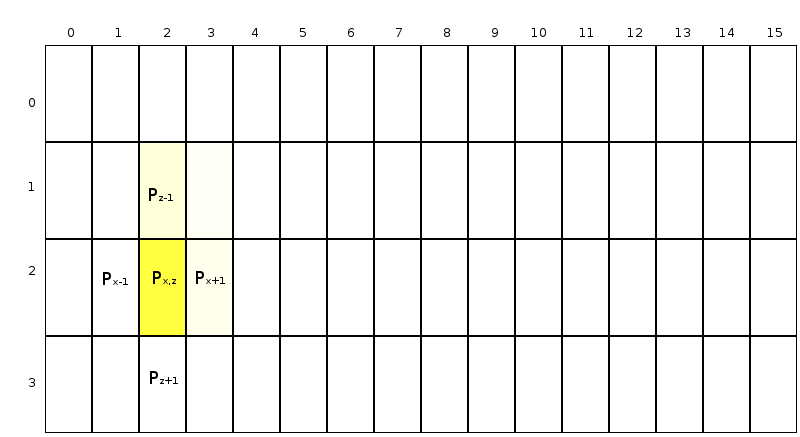
\includegraphics[scale=0.5]{figs/PixelGrid.png}
\caption{
The pixels on the Cassini VIMS instrument are 0.5x0.25 milliradians for images
taken in high-resolution mode. They are 0.5x0.5 milliradians for images taken
in low-resolution mode. This is a diagram of the instrument field-of-view for a
16x4 high-resolution imaging-mode occultation, such as that for the AlpOri
occultation of rev270s99. The pixels used in the calculation of the metric $R$
are labeled.
}
\label{fig:pixels}
\end{figure}

\section{Selecting the Comparison Pixel}

We calculate the brightest pixel, $P^x=P^z$, using the brightest pixel
algorithm described in the code document. Then we mark "transitions" when the
brightest pixel moves from one position to the next. We use the position of the
brightest pixel beyond the nearest transition as the comparison pixel. See the
code document for the full write-up, or I should combine these documents at
some point (likely).

The background-corrected brightness of these two pixels is divided to arrive at
$R_{data}$

\section{The Metric}

We measure the direction to the star by modeling which two pixels might be
sharing starlight, then taking the ratio of their de-noised signal $R_{data}$.
We compare this ratio to the same ratio calculated from the PRF scans
$R_{scans}(t)$ at each time step $t$. We calculate the value of $t=t_0$ for
which $\chi^2 = (R_{data}-R_{scans}(t_0))^2$ is minimized, and then calculate
$\theta(t_0)$ which is the offset of the star from the center of the pixel at
$t_0$.

\begin{equation}
R_{data}^x = \frac{P^{x\pm1}}{P^{x}}
\end{equation}

And in the $z$ direction this ratio is defined as:

\begin{equation}
R_{data}^z = \frac{P^{z\pm1}}{P^{z}}
\end{equation}

Where $P^x = P^z$ is the brightness of the brightest pixel (integrated over
some wavelength range), and $P^{x\pm1}$ and $P^{z\pm1}$ are those of the
adjacent pixels in each direction, as shown in Figure \ref{fig:pixels}.

This metric has many properties which make it useful. Theoretically, it should
be monotonically increasing or decreasing as the star position increases
steadily in pixel position.  For PSFs smaller than a pixel, there will be a
plateau at zero where there is no light observed in the neighboring pixel. Away
from this plateau (near the pixel boundaries) we have the best sensitivity to
the position of the star. At metric values $R = 1$ the center of the star's PSF
straddles the boundary with the neighboring pixel and we have the most
sensitivity.

\section{The Pixel Scans}

We have scans of the sensitivity of VIMS's spatial pixel as a function of the
position of the star relative to the center of the pixel created by slewing the
spacecraft around in a raster-scan pattern as shown in Figure \ref{fig:scans}.

\begin{figure}[h!]
\centering
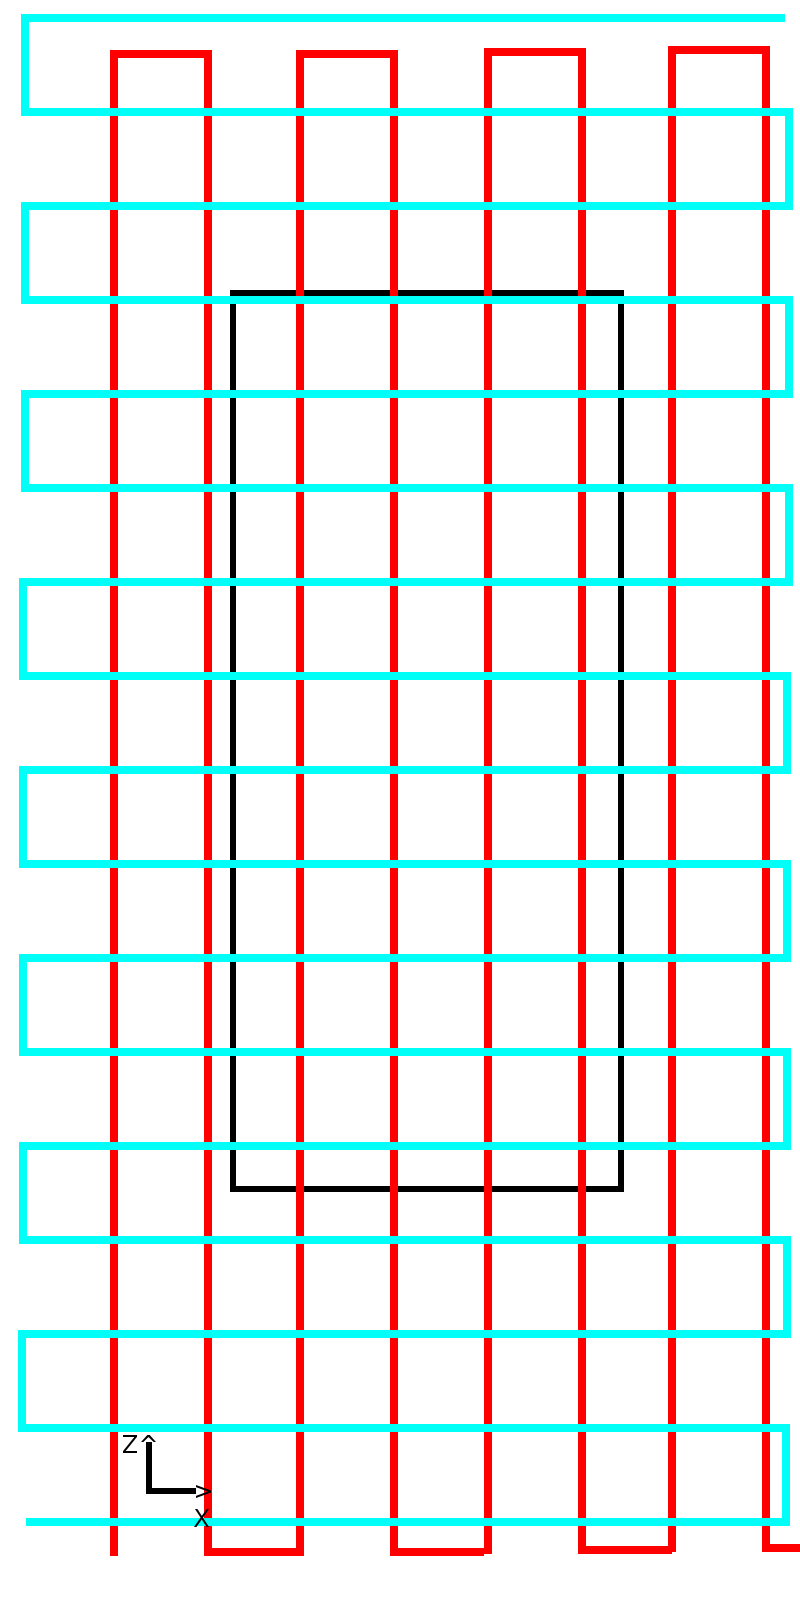
\includegraphics[scale=0.3]{figs/ScanLines.png}
\caption{
Black Box is pixel, Red scans are Z scans, Cyan scans are X scans.
The spacecraft was slewed such that the center of the star passed along the
paths shown by the scan-lines.
}
\label{fig:scans}
\end{figure}

{\em \bf NOTES:} I am currently only using x-scan 7 (near the middle), and only
for the observations where the spacecraft's motion was aligned with the x-axis.
These central scans saturate the pixel at the very shortest wavelengths. This
impacts one of the observed band-passes in my code. I have plans to select the
best scan in each direction that I need to develop further.

\section{Calculating the Theoretical Metric from the Scans}

One of the most well-constrained and precisely repeatable parts of the VIMS
camera is the interpixel distance, $\theta_{pix}$ (Phil Nicholson, private
communication).  Therefore, we should be able to reliably calculate the
theoretical metric along a scanline from the scanned data using the following
formula:

\begin{equation}
  R_{scans}(t) = \frac{PRF(t\pm\frac{\theta_{pix}}{\dot\theta_{spacecraft}})}{PRF(t)}
\end{equation}

where $\theta_{pix}$ is the fixed interpixel distance and $\dot\theta_{spacecraft}$
is the fixed spacecraft velocity during the scan.

The buffer provided in each scan provides a domain of the metric that extends
beyond the edge of the pixel so that we can still test those values for
completeness of the fitting algorithm described in the next section.

\section{Fitting the Experimental Metric to the Theoretical}

Now we have a map of the metric along each scan extending beyond the edges of
each pixel, and the observed value of the metric.

Next, we calculate the $t_0$ for which $\chi^2 = (R_{data}-R_{scans}(t_0))^2$
is minimized, and then calculate $\theta(t_0)$ which is the offset from the
center of the pixel at $t_0$.

\section{Results}

In Figure \ref{fig:results}, you can see the results of one of these centering
runs for the occultation AlpOri271S99.

\begin{figure}[h!]
\centering
\includegraphics[scale=0.2]{figs/AlpOri271S99.png}
\caption{
    (top)
    Occultation light curve as AlpOri passed behind Saturn from the vantage point of Cassini VIMS on rev 271.\\
    (bottom)
    In green, you can see the step-wise brightest pixel centering that had resolution of one pixel.
    In red, you can see the centering calculated as a result of the algorithm described in this paper.
    The plus signs mark where the transitionfinder() function marked pixel transitions.
    The black line marks the calculated position of the limb of Saturn, which is where the refracted light should appear to come from.
}
\label{fig:results}
\end{figure}



\end{document}
This is never printed
